\chapter{Équation d’état, rayonnement et énergie du vide}

\lectureoverview{L’histoire d’un univers homogène est en grande partie celle de son facteur d’échelle \(a(t)\). L’équation de Friedmann fournit la géométrie, mais c’est l’équation d’état de la matière qui indique comment la densité d’énergie évolue pendant l’expansion de l’espace. Nous allons d’abord déduire \(\rho\propto a^{-3(1+w)}\) à partir du travail effectué par un fluide, puis établir \(P=\rho/3\) pour le rayonnement en comptant les transferts de quantité de mouvement des photons, et enfin caractériser l’énergie du vide par \(P=-\rho\). Une énergie du vide positive produit une expansion de de Sitter ; la courbure et le signe de la constante cosmologique donnent des solutions avec rebond ou effondrement, que l’on peut interpréter comme de simples systèmes mécaniques.}

\section{Le facteur d’échelle et la loi manquante pour la matière}

Rappelons d’abord où nous en sommes. Dans l’approximation d’un univers homogène et isotrope, l’essentiel de l’histoire cosmologique est décrit par une seule fonction, \(a(t)\). La connaître ne répond pas à toutes les questions sur l’univers, mais elle détermine les distances, les taux d’expansion et la succession des grandes ères cosmologiques. Cette leçon ne vise pas encore à établir ces ères à partir des observations. Elle consiste à déduire, à partir de la physique fondamentale, les équations d’état qui rendent les modèles possibles.

Deux modèles de référence sont déjà apparus :
\begin{equation}
a(t)\propto t^{2/3}
\qquad\text{(matter domination)},
\end{equation}
et
\begin{equation}
a(t)\propto t^{1/2}
\qquad\text{(radiation domination)}.
\end{equation}
Aucune de ces lois n’est exacte à toutes les époques. Le rayonnement fournit une approximation utile aux premiers temps et la matière, une approximation valable plus tard, pendant une période intermédiaire ; l’énergie du vide modifie ensuite le comportement aux temps tardifs. La question immédiate n’est pas de savoir comment les observations révèlent ces ères, mais ce qui distingue les membres de droite correspondants dans l’équation de Friedmann.

\begin{figure}[htbp]
\centering
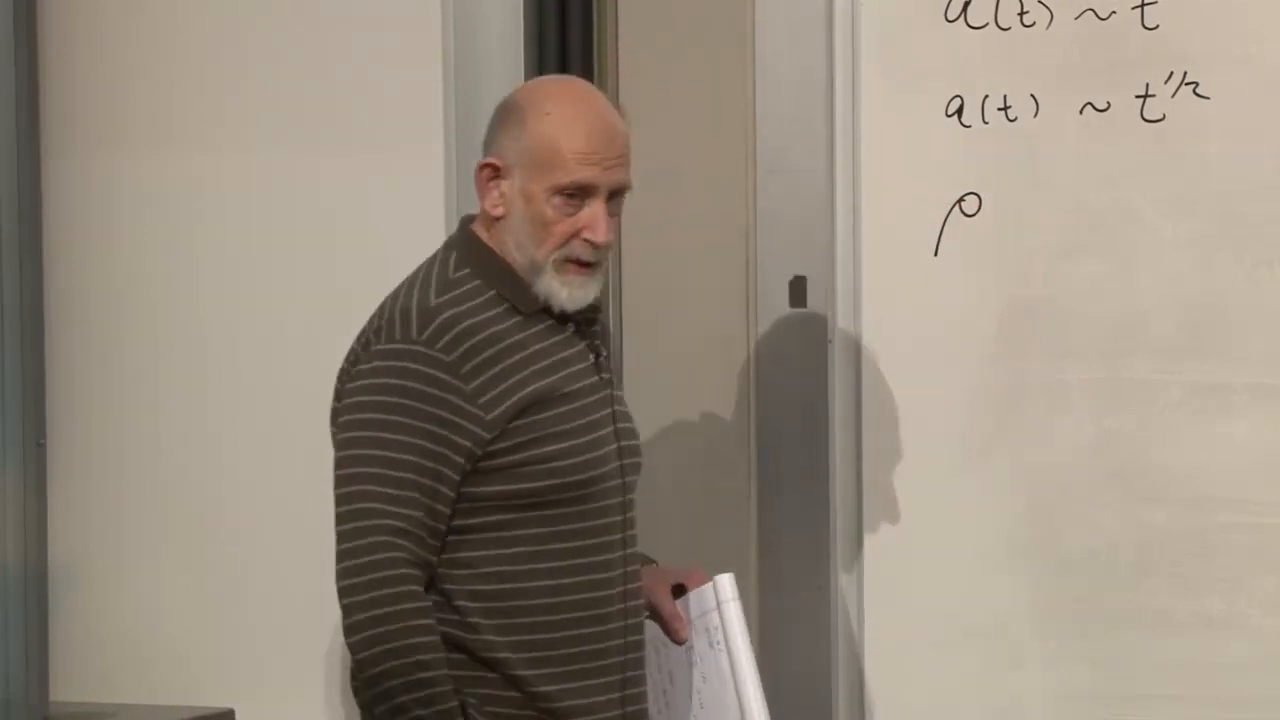
\includegraphics[width=0.72\textwidth]{lecture_05_figure_02.png}
\caption{Lois de puissance du facteur d’échelle rappelées et symbole de densité nouvellement introduit. Il s’agit d’un état transitoire du tableau, et non d’une démonstration achevée.}
\label{fig:c05-review-board}
\lectureframe{00:03:18.380}
\end{figure}

Le chaînon manquant est l’équation d’état. Elle détermine comment la densité d’énergie figurant au membre de droite de l’équation de Friedmann varie avec le facteur d’échelle. Les deux lois de référence sont
\begin{equation}
\rho_{\text{matter}}=\frac{\rho_0}{a^3},
\qquad
\rho_{\text{rad}}=\frac{\rho_0}{a^4}.
\label{eq:c05-benchmark-densities}
\end{equation}
La matière se dilue comme le volume, lequel varie comme \(a^3\). La densité de rayonnement décroît avec une puissance supplémentaire de \(a\). Nous voulons comprendre ces deux lois à partir de la relation entre pression et densité d’énergie.

\section{De la pression à la loi d’évolution de la densité}

Une équation d’état peut en général faire intervenir la densité, la pression, la température et d’autres variables. Pour les composantes cosmologiques étudiées ici, adoptons la forme utile à paramètre constant \(w\) :
\begin{equation}
P=w\rho,
\label{eq:c05-eos}
\end{equation}
où \(w\) caractérise le fluide. Le tableau utilise la majuscule \(W\) ; nous adoptons la minuscule conventionnelle \(w\). Cette forme linéaire couvre les cas importants qui suivent, mais c’est une hypothèse simplificatrice, et non une loi vérifiée par tous les fluides possibles.

Pour la matière non relativiste, la densité d’énergie est dominée par l’énergie de masse au repos. Si \(n\) est la densité numérique et \(m\) la masse des particules, on a schématiquement
\begin{equation}
\rho\simeq nmc^2.
\end{equation}
Le facteur \(c^2\) fait d’une masse au repos, même faible, une réserve d’énergie énorme ; l’annihilation complète d’un grain de poussière libérerait une quantité d’énergie macroscopique. La pression, en revanche, résulte des transferts de quantité de mouvement lorsque les particules heurtent une paroi et est de l’ordre de \(nmv^2\). Une boule de bowling transfère plus de quantité de mouvement qu’une balle de ping-pong, mais, dans un gaz froid, toute vitesse pertinente vérifie \(v\ll c\). On a donc
\begin{equation}
\frac{P}{\rho}\sim\frac{v^2}{c^2}\ll1,
\qquad
w\simeq0.
\label{eq:c05-dust-eos}
\end{equation}
Le rayonnement se déplace à \(c\) ; cette approximation ne s’applique donc pas à lui. Nous allons déduire sa valeur de \(w\) au lieu de la supposer.

Il nous faut maintenant une méthode générale pour transformer l’équation~\eqref{eq:c05-eos} en loi d’évolution de \(\rho\). Une boîte de laboratoire suffit. On ne peut pas littéralement placer des galaxies dans une boîte, mais après lissage elles se comportent comme des particules, et la relation entre énergie et pression peut se déduire localement.

\begin{figure}[htbp]
\centering
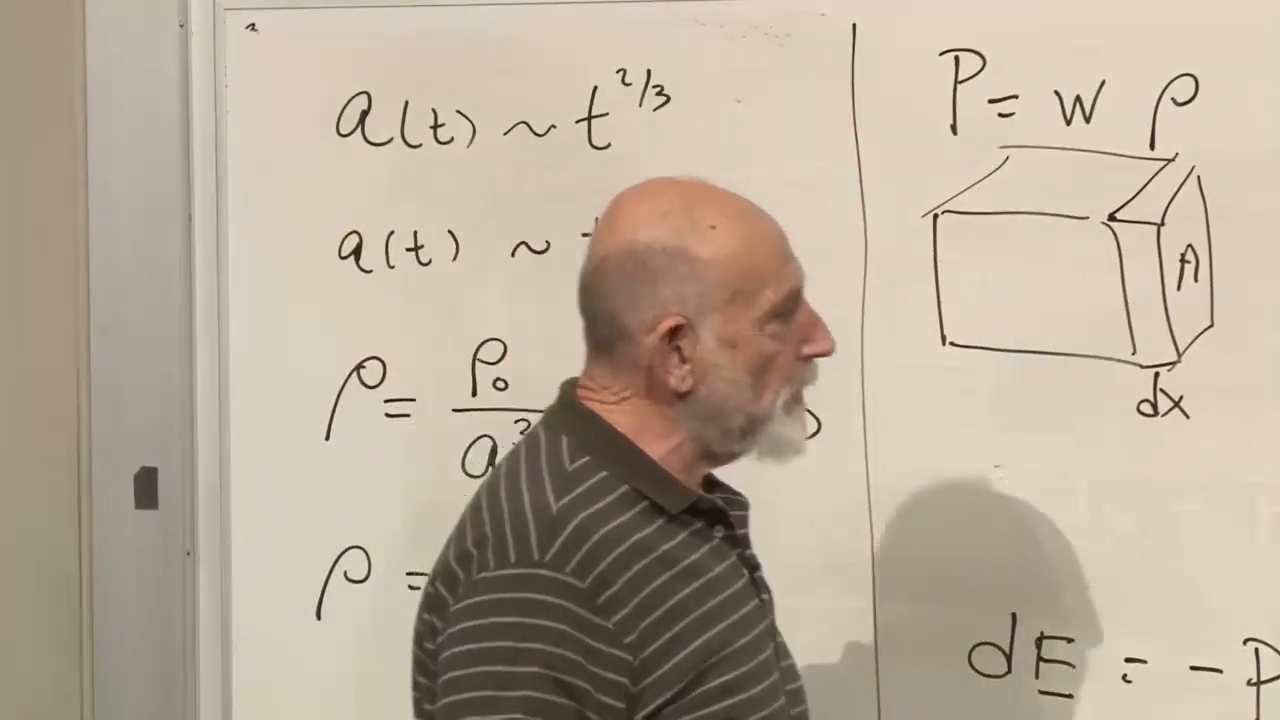
\includegraphics[width=0.86\textwidth]{lecture_05_figure_03.png}
\caption{L’équation d’état, les lois d’évolution de la densité rappelées et la boîte thermodynamique figurent sur un même tableau. Le conférencier masque une partie des inscriptions précédentes ; l’image sert donc à montrer la disposition et les équations visibles, plutôt qu’à fournir une transcription complète.}
\label{fig:c05-box-board}
\lectureframe{00:13:39.612}
\end{figure}

À gauche du tableau figurent les lois cosmologiques rappelées ; à droite commence l’argument de la boîte. Pris ensemble, les éléments visibles relient
\begin{equation}
\rho_{\text{matter}}=\frac{\rho_0}{a^3},
\qquad
\rho_{\text{rad}}=\frac{\rho_0}{a^4},
\qquad
P=w\rho.
\end{equation}
Nous devons déduire les deux lois de densité à partir de l’équation d’état.

Une paroi a pour aire \(A\). Déplaçons-la vers l’extérieur de \(dx\), de sorte que
\begin{equation}
dV=A\,dx.
\end{equation}
La pression étant la force par unité de surface, la force exercée sur la paroi vaut \(PA\). Le gaz fournit le travail \(PA\,dx=P\,dV\), et l’énergie qui reste à l’intérieur diminue.
\begin{equation}
dE=-P\,dV.
\label{eq:c05-work-law}
\end{equation}
\begin{figure}[htbp]
\centering
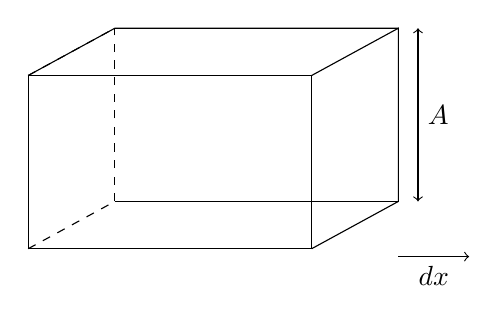
\begin{tikzpicture}[scale=1.0]
\draw (0,0) -- (3.6,0) -- (3.6,2.2) -- (0,2.2) -- cycle;
\draw (3.6,0) -- (4.7,0.6) -- (4.7,2.8) -- (3.6,2.2);
\draw (0,2.2) -- (1.1,2.8) -- (4.7,2.8);
\draw (1.1,0.6) -- (4.7,0.6);
\draw[dashed] (0,0) -- (1.1,0.6);
\draw[dashed] (0,2.2) -- (1.1,2.8);
\draw[dashed] (1.1,0.6) -- (1.1,2.8);
\draw[<->] (4.95,0.6) -- (4.95,2.8);
\node[right] at (4.95,1.7) {\(A\)};
\draw[->] (4.7,-0.1) -- (5.6,-0.1);
\node[below] at (5.15,-0.1) {\(dx\)};
\end{tikzpicture}
\caption{Reconstitution nette de la boîte thermodynamique, avec une face d’aire \(A\) et un déplacement \(dx\).}
\label{fig:c05-box-redraw}
\end{figure}

L’énergie totale est
\begin{equation}
E=\rho V.
\end{equation}
En dérivant, on obtient
\begin{equation}
d(\rho V)=\rho\,dV+V\,d\rho.
\end{equation}
En substituant dans l’équation~\eqref{eq:c05-work-law}, on trouve
\begin{equation}
\rho\,dV+V\,d\rho=-P\,dV.
\end{equation}
Insérons \(P=w\rho\) :
\begin{equation}
V\,d\rho=-(1+w)\rho\,dV.
\end{equation}
On approche de l’équation utile, mais il manque encore une étape. Divisons par \(\rho V\).
\begin{equation}
\frac{d\rho}{\rho}=-(1+w)\frac{dV}{V}.
\end{equation}
\begin{figure}[htbp]
\centering
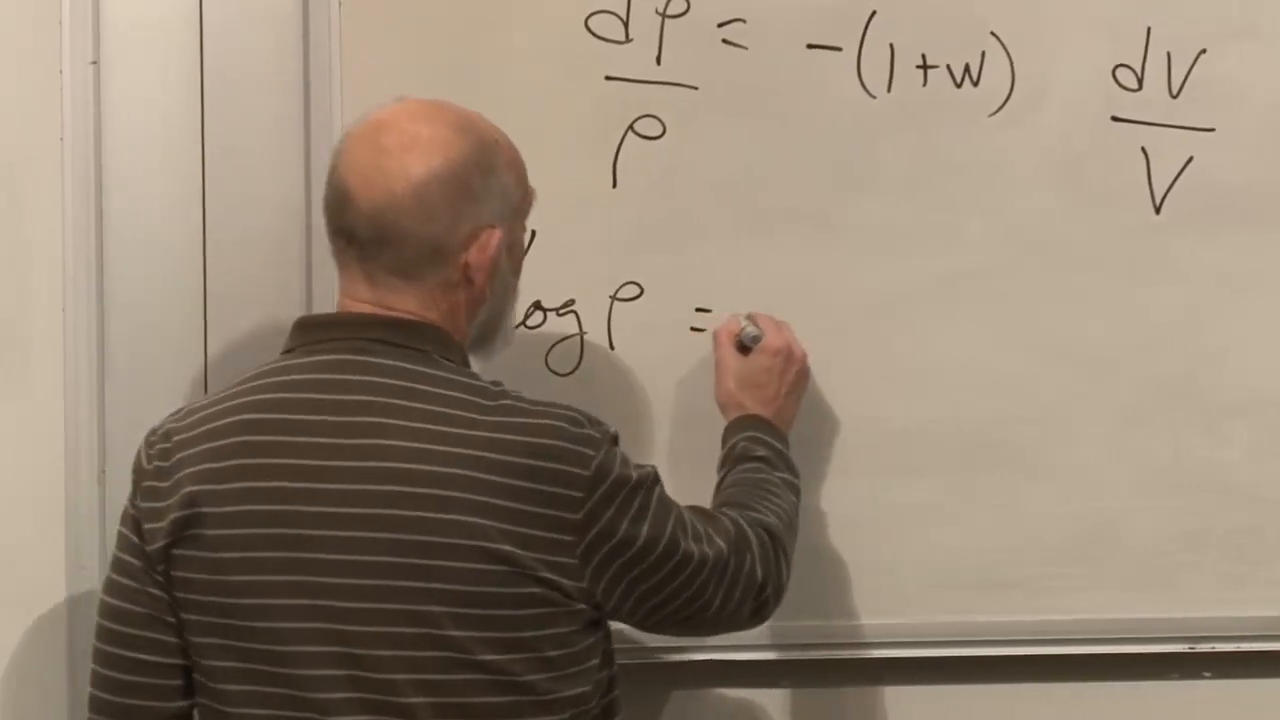
\includegraphics[width=0.78\textwidth]{lecture_05_figure_04.png}
\caption{Équation séparée reliant la densité au volume et début de l’intégration logarithmique. Le membre de droite complet est reconstitué à partir du calcul précédent, et non déduit des pixels masqués.}
\label{fig:c05-log-board}
\lectureframe{00:15:35.600}
\end{figure}

L’image montre l’équation séparée et le début de \(\log\rho=\). Achevons directement l’intégration :
\begin{equation}
d(\log\rho)=-(1+w)\,d(\log V),
\end{equation}
de sorte que
\begin{equation}
\log\rho=-(1+w)\log V+\text{const.}
\end{equation}
En prenant l’exponentielle,
\begin{equation}
\rho\propto V^{-(1+w)}.
\end{equation}
C’est la loi reliant la densité au volume.

Revenons maintenant de la boîte à la cosmologie. Le déplacement d’une seule paroi était une commodité de calcul, et non une hypothèse d’anisotropie. Une expansion uniforme dans les trois directions donne la même relation de travail, et un volume comobile varie comme
\begin{equation}
V\propto a^3.
\end{equation}
Par conséquent,
\begin{equation}
\boxed{\rho\propto a^{-3(1+w)}}.
\label{eq:c05-density-scaling}
\end{equation}
En \(d\) dimensions spatiales, l’exposant \(3\) deviendrait \(d\) ; le reste du raisonnement serait inchangé.

\section{Premières applications : matière et rayonnement}

Nous pouvons maintenant retrouver les formules récapitulatives en les déduisant, plutôt qu’en les postulant.

Pour la matière non relativiste, prenons
\begin{equation}
w=0.
\end{equation}
Alors,
\begin{equation}
\rho\propto a^{-3},
\end{equation}
ce qui donne exactement la loi de dilution de la matière.

Pour le rayonnement, prenons provisoirement
\begin{equation}
w=\frac13.
\end{equation}
Si cette hypothèse est correcte, alors
\begin{equation}
\rho\propto a^{-3(1+1/3)}=a^{-4}.
\end{equation}
La puissance inverse supplémentaire équivaut donc à \(w=1/3\). Il reste à déduire cette valeur de la physique des photons.

\section{Pourquoi la pression du rayonnement vaut un tiers de sa densité d’énergie}

Le rayonnement peut être décrit comme des ondes électromagnétiques ou comme des particules sans masse. Utilisons les photons pour calculer la pression d’un gaz de photons dans une boîte. La boîte est représentée en deux dimensions, mais le gaz et sa distribution angulaire sont tridimensionnels. Les photons se déplacent à la vitesse de la lumière et rebondissent élastiquement sur les parois idéalisées pour le calcul.

Pour l’instant, supposons que tous les photons ont la même énergie \(\epsilon\). Cette simplification disparaîtra lorsque nous additionnerons les contributions d’énergies différentes. Soit \(\vec{\pi}\) le vecteur quantité de mouvement d’un photon ; évitons la notation usuelle \(p\), puisque \(P\) désigne déjà la pression. Une particule sans masse obéit aux relations suivantes.
\begin{equation}
\epsilon=c\,\pi,
\end{equation}
avec \(\pi=|\vec{\pi}|\). Dans le système d’unités utilisé dans cette leçon, \(c=1\), donc
\begin{equation}
\epsilon=\pi.
\end{equation}
Si \(\nu\) est la densité numérique de photons, la densité d’énergie vaut
\begin{equation}
\rho=\epsilon\,\nu.
\end{equation}
Considérons une paroi dont la normale est dirigée selon l’axe \(x\). Pendant un bref intervalle \(\Delta t\), un photon se déplaçant selon un angle \(\theta\) par rapport à cette normale n’atteint la paroi que s’il se trouve initialement dans une tranche d’épaisseur
\begin{equation}
\Delta x=\Delta t\cos\theta.
\end{equation}
Lors de la réflexion, sa composante \(x\) de la quantité de mouvement change de signe ; la quantité de mouvement transférée à la paroi vaut donc
\begin{equation}
\Delta \pi_x=2\epsilon\cos\theta.
\end{equation}
La force étant le transfert de quantité de mouvement par unité de temps, chaque impact contribue \(\Delta \pi_x/\Delta t\). La tranche contient \(\nu A\Delta x\) photons, mais seule la moitié se dirige vers la paroi ; le nombre pertinent est donc \(\tfrac12 \nu A\Delta x\). En divisant la force totale par l’aire de la paroi \(A\), on obtient
\begin{align}
P(\theta)
&=
\frac{1}{A}
\left(\frac{2\epsilon\cos\theta}{\Delta t}\right)
\left(\frac12 \nu A\Delta x\right) \\
&=
\epsilon\nu\cos\theta\frac{\Delta x}{\Delta t} \\
&=
\epsilon\nu\cos^2\theta \\
&=
\rho\cos^2\theta.
\end{align}
Le résultat dépend de l’angle, car il ne tient compte que de la contribution des photons se déplaçant dans une seule direction.

\begin{figure}[htbp]
\centering
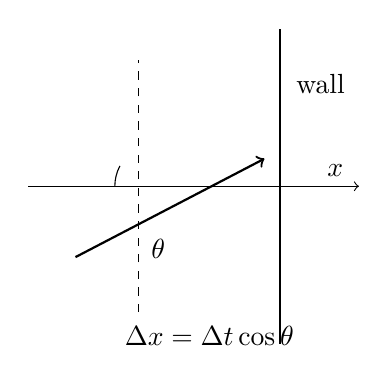
\begin{tikzpicture}[scale=1.0]
\draw[thick] (0,0) -- (0,4);
\draw[->] (-3.2,2) -- (1.0,2);
\node[above] at (0.7,2) {\(x\)};
\draw[dashed] (-1.8,0.4) -- (-1.8,3.6);
\node[below] at (-0.9,0.35) {\(\Delta x=\Delta t\cos\theta\)};
\draw[->,thick] (-2.6,1.1) -- (-0.2,2.35);
\node[below] at (-1.55,1.45) {\(\theta\)};
\draw (-2.1,2) arc[start angle=180,end angle=152,radius=0.55];
\node[right] at (0.08,3.3) {wall};
\end{tikzpicture}
\caption{Quantité de mouvement d’un photon incident sur une paroi sous un angle \(\theta\) ; géométrie utilisée pour déduire la pression du rayonnement.}
\label{fig:c05-photon-pressure}
\end{figure}

Faisons la moyenne sur la distribution isotrope. Soit \(\mathbf n=(n_x,n_y,n_z)\) le vecteur unitaire dirigé selon la direction d’un photon. Alors,
\begin{equation}
n_x=\cos\theta,
\qquad
n_x^2+n_y^2+n_z^2=1.
\end{equation}
Dans un gaz isotrope, les moyennes de \(n_x^2\), \(n_y^2\) et \(n_z^2\) sont égales. En prenant la moyenne de l’identité ci-dessus,
\begin{equation}
\langle n_x^2\rangle+\langle n_y^2\rangle+\langle n_z^2\rangle=1,
\end{equation}
et, par symétrie, chaque terme étant identique, on obtient
\begin{equation}
\langle n_x^2\rangle=\langle \cos^2\theta\rangle=\frac13.
\end{equation}
Par conséquent,
\begin{equation}
P=\rho\langle \cos^2\theta\rangle=\frac{\rho}{3}.
\end{equation}
L’équation d’état du rayonnement est donc
\begin{equation}
P=\frac13\rho,
\qquad
w=\frac13.
\end{equation}
Le facteur \(1/3\) correspond au nombre de directions spatiales qui se partagent le carré du vecteur unitaire. Dans \(d\) dimensions spatiales isotropes, le même raisonnement donnerait \(\langle n_x^2\rangle=1/d\). Nous achevons ainsi la démonstration microscopique annoncée au début.

\subsection{Questions pour vérifier le raisonnement sur le rayonnement}

\begin{classroomqa}
\audiencequestion{Tous les photons doivent-ils avoir la même énergie ?}
\lecturerresponse{Non. Effectuons le calcul séparément pour chaque intervalle d’énergie. Chaque intervalle contribue à la pression à hauteur du tiers de sa propre densité d’énergie ; la somme sur le spectre conserve donc \(P=\rho/3\). L’hypothèse d’une énergie identique ne servait qu’à alléger les notations. \lecturetimestamp{00:39:08--00:39:36}}
\end{classroomqa}

\begin{classroomqa}
\audiencequestion{Des parois noires absorbantes donneraient-elles le même résultat que des miroirs parfaits, et que représente la paroi dans l’espace vide ?}
\lecturerresponse{Une paroi noire à l’équilibre thermique absorbe le rayonnement puis le réémet, ce qui produit le même bilan moyen de quantité de mouvement. L’espace cosmologique n’a pas de paroi réelle ; la surface est une frontière imaginaire. Pour chaque photon qui la traverse vers l’extérieur, l’isotropie fournit un flux moyen compensateur vers l’intérieur ; le calcul local du flux de quantité de mouvement reste donc inchangé. Le rayonnement étudié en cours est principalement le fond diffus cosmologique thermique, pour lequel cette représentation par l’équilibre est particulièrement naturelle. \lecturetimestamp{00:39:37--00:41:19}}
\end{classroomqa}

\begin{classroomqa}
\audiencequestion{Les statistiques quantiques modifient-elles \(P=\rho/3\)?}
\lecturerresponse{Non. La statistique de Bose détermine la façon dont les photons occupent les modes disponibles et, par conséquent, le spectre et la valeur totale de \(\rho\), mais la contrainte isotrope de particules sans masse reste égale au tiers de cette densité d’énergie. \lecturetimestamp{00:41:51--00:42:02}}
\end{classroomqa}

\begin{classroomqa}
\audiencequestion{Que se passe-t-il si les photons se diffusent les uns sur les autres ?}
\lecturerresponse{La diffusion ordinaire entre photons est extrêmement faible ; sa correction est donc négligeable ici. À température et densité suffisamment élevées, les collisions peuvent créer des paires électron-positon et modifier le contenu effectif en particules ainsi que l’équation d’état. C’est un effet réel, mais il concerne un régime bien plus chaud que celui considéré dans ce raisonnement. \lecturetimestamp{00:42:02--00:43:08}}
\end{classroomqa}

\begin{classroomqa}
\audiencequestion{Qu’est devenue l’aire de la paroi \(A\)?}
\lecturerresponse{Le produit intermédiaire est la force exercée par un photon multipliée par le nombre de photons qui frappent la paroi ; ce nombre est proportionnel à \(A\). La pression étant la force divisée par l’aire, la division finale par \(A\) s’annule. L’omission au tableau consistait à appeler trop tôt pression l’expression intermédiaire ; rétablir l’étape qui fait passer de la force à la pression corrige le calcul. \lecturetimestamp{00:43:11--00:44:01}}
\end{classroomqa}

\section{Pression négative et sens de la tension}

Jusqu’ici, les particules ont heurté les parois et les ont poussées vers l’extérieur. Cette représentation produit naturellement une pression positive, mais elle ne couvre pas tous les cas possibles.

\begin{classroomqa}
\audiencequestion{La densité d’énergie elle-même peut-elle être négative ?}
\lecturerresponse{La théorie quantique autorise des densités d’énergie négatives dans certaines circonstances restreintes, et la constante cosmologique peut formellement avoir l’un ou l’autre signe. Ces cas demandent de la prudence et ne constituent pas notre point de départ immédiat. La possibilité plus familière est celle d’une \emph{pression négative}, qui peut survenir même lorsque la densité d’énergie est positive. \lecturetimestamp{00:44:25--00:44:59}}
\end{classroomqa}

\begin{classroomqa}
\audiencequestion{Comment une pression peut-elle être négative ?}
\lecturerresponse{Dans un monde à une dimension, une boîte est un segment de droite. Des particules en mouvement libre rebondissent sur ses extrémités et les poussent vers l’extérieur, ce qui donne une pression positive. Relions plutôt les extrémités par une corde tendue ou un ressort. Si l’on écarte les extrémités, le ressort tire dessus vers l’intérieur. Cette force dirigée vers l’intérieur est une tension ; elle représente la pression négative dans le modèle à une dimension. \lecturetimestamp{00:45:04--00:46:31}}
\end{classroomqa}

\begin{figure}[htbp]
\centering
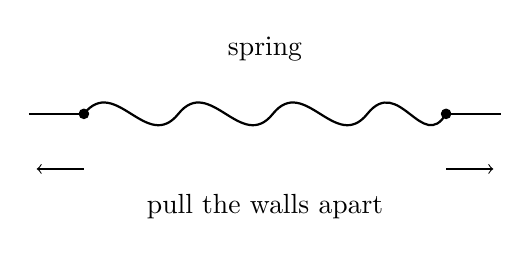
\begin{tikzpicture}[scale=1.0]
\draw[thick] (-3,0) -- (-2.3,0);
\draw[thick] (2.3,0) -- (3,0);
\draw[fill] (-2.3,0) circle (0.06);
\draw[fill] (2.3,0) circle (0.06);
\draw[thick] (-2.3,0)
.. controls (-1.9,0.5) and (-1.5,-0.5) .. (-1.1,0)
.. controls (-0.7,0.5) and (-0.3,-0.5) .. (0.1,0)
.. controls (0.5,0.5) and (0.9,-0.5) .. (1.3,0)
.. controls (1.7,0.5) and (2.0,-0.5) .. (2.3,0);
\draw[->] (-2.3,-0.7) -- (-2.9,-0.7);
\draw[->] (2.3,-0.7) -- (2.9,-0.7);
\node[below] at (0,-0.9) {pull the walls apart};
\node[above] at (0,0.55) {spring};
\end{tikzpicture}
\caption{Un ressort unidimensionnel, par analogie avec la pression négative.}
\label{fig:c05-tension}
\end{figure}

Le bilan des travaux s’inverse en conséquence. Lorsqu’un gaz à pression positive se dilate, il fournit un travail et perd de l’énergie interne. Écarter les extrémités contre la tension emmagasine de l’énergie dans le ressort. Plus généralement, des constituants attractifs peuvent s’attirer mutuellement et attirer la frontière vers l’intérieur. Un système peut donc avoir \(\rho>0\) et \(P<0\), d’où \(w<0\), sans aucune contradiction. Cette possibilité est essentielle, car l’énergie du vide présente précisément ce jeu de signes.

\section{Énergie du vide et constante cosmologique}

On attribue l’énergie du vide à l’espace vide lui-même. La théorie quantique des champs la motive par le mouvement de point zéro des oscillateurs harmoniques associés aux modes des champs, mais sa description macroscopique ne nous oblige pas à résoudre ce problème microscopique. Sa propriété définissante est que l’espace vide possède la même densité d’énergie, quel que soit l’endroit ou le volume de la région choisie.
\begin{equation}
\rho=\rho_0=\text{const.}
\label{eq:c05-vacuum-density}
\end{equation}
Si une région de volume \(V\) ne contient que de l’énergie du vide, son énergie totale vaut
\begin{equation}
E=\rho_0 V.
\end{equation}
\begin{classroomqa}
\audiencequestion{Une boîte modifie-t-elle la densité du vide en limitant les modes de champ autorisés ?}
\lecturerresponse{L’énergie totale d’une région finie est inférieure à celle de tout l’espace, car son volume est plus petit ; la densité moyenne \(\rho_0\) reste la même. De véritables frontières peuvent modifier les énergies des modes et produire l’effet Casimir, mais cette correction compte lorsque les séparations sont comparables aux longueurs d’onde pertinentes. Elle n’est pas la densité du vide à grande échelle utilisée en cosmologie. \lecturetimestamp{00:50:06--00:51:25}}
\end{classroomqa}

Introduisons
\begin{equation}
\Lambda=\frac{8\pi G}{3}\rho_0.
\label{eq:c05-lambda-definition}
\end{equation}
Cette définition regroupe les facteurs qui apparaissent dans l’équation de Friedmann. La relation inverse est
\begin{equation}
\rho_0=\frac{3\Lambda}{8\pi G}.
\end{equation}
Le paramètre \(\Lambda\) est la constante cosmologique. On appelle couramment énergie noire une composante positive, presque constante, qui entraîne l’accélération tardive de l’expansion.

La dépendance en facteur d’échelle étant déjà établie, reprenons le raisonnement de la boîte à rebours pour déterminer la pression. Puisque \(d\rho_0=0\),
\begin{equation}
dE=d(\rho_0V)=\rho_0\,dV.
\end{equation}
Par ailleurs, la relation thermodynamique entre travail et énergie reste
\begin{equation}
dE=-P\,dV.
\end{equation}
En posant \(P=w\rho_0\), on obtient
\begin{equation}
dE=-w\rho_0\,dV.
\end{equation}
La comparaison donne
\begin{equation}
w=-1.
\end{equation}
et donc
\begin{equation}
P=-\rho.
\end{equation}
L’analogie du ressort annonçait ce signe. Une énergie du vide positive a une pression négative ; une énergie du vide négative a une pression positive. Les mesures astronomiques de \(w\) cherchent à savoir si la composante tardive se comporte réellement comme un vide qui ne se dilue pas : plus \(w\) est proche de \(-1\), plus son comportement se rapproche de l’équation~\eqref{eq:c05-vacuum-density}.

\begin{classroomqa}
\audiencequestion{Est-ce que \(P=-\rho\) est l’équation d’état d’un univers vide, et peut-on calculer \(\rho_0\)?}
\lecturerresponse{C’est l’équation d’état de l’espace vide lorsqu’il contient de l’énergie du vide. En revanche, il est beaucoup plus difficile d’en déterminer la valeur absolue. Tous les champs quantiques et toutes les échelles d’énergie peuvent contribuer, y compris ceux qui n’ont pas encore été découverts ; aucun calcul admis n’explique donc la valeur observée. Le principal mystère n’est pas d’écrire \(w=-1\), mais de comprendre pourquoi la valeur nette de \(\rho_0\) est si extraordinairement faible. \lecturetimestamp{00:57:27--00:58:29}}
\end{classroomqa}

\section{L’énergie du vide dans la dynamique de Friedmann}

Isolons l’énergie du vide, comme nous l’avons fait précédemment pour la matière seule et le rayonnement seul. Avec \(\rho=\rho_0\), l’équation de Friedmann devient
\begin{equation}
\left(\frac{\dot a}{a}\right)^2=\Lambda-\frac{k}{a^2},
\label{eq:c05-vacuum-friedmann}
\end{equation}
où \(k=+1,0,-1\) pour les espaces sphérique, plat et hyperbolique. Les signes positif et négatif de \(\Lambda\), combinés aux trois choix de \(k\), donnent six cas de signe, même si certains n’admettent aucune solution réelle.

\begin{remark}
Dans cette leçon, \(\Lambda=(8\pi G/3)\rho_0\), si bien que \(\Lambda\) a ici les dimensions de \(H^2\). Avec la convention courante \(G_{\mu\nu}+\Lambda_{\mathrm E}g_{\mu\nu}=8\pi G T_{\mu\nu}\), le paramètre correspondant est \(\Lambda_{\mathrm E}=3\Lambda\).
\end{remark}

\subsection{Expansion plate de de Sitter}

Posons \(k=0\). Alors,
\begin{equation}
\left(\frac{\dot a}{a}\right)^2=\Lambda.
\end{equation}
Pour \(\Lambda>0\), choisissons la branche en expansion :
\begin{equation}
\dot a=\sqrt{\Lambda}\,a,
\end{equation}
et donc
\begin{equation}
a(t)=C\,e^{\sqrt{\Lambda}\,t}.
\end{equation}
Le paramètre de Hubble est alors constant :
\begin{equation}
H=\frac{\dot a}{a}=\sqrt{\Lambda}.
\end{equation}
Il s’agit de l’espace de de Sitter en coordonnées plates, nommé d’après Willem de Sitter, qui a trouvé la solution avec constante cosmologique peu après qu’Einstein a introduit ce terme en 1917. Si \(\Lambda<0\) alors que \(k=0\), l’équation~\eqref{eq:c05-vacuum-friedmann} n’a pas de solution réelle, car \(H^2\) ne peut pas être négatif.

\begin{classroomqa}
\audiencequestion{Le paramètre de Hubble est-il vraiment constant ici, et cet espace-temps a-t-il un big bang ?}
\lecturerresponse{Pour la solution pure en coordonnées plates, \(H=\sqrt{\Lambda}\) est exactement constant. Bien que \(a(t)\to0\) seulement lorsque \(t\to-\infty\), cette carte de coordonnées n’est pas géodésiquement complète : certaines trajectoires orientées vers le passé atteignent sa frontière en un temps propre fini. La formule ne permet donc pas, à elle seule, de trancher la question du big bang global. La géométrie complète de de Sitter ne se limite pas à cette carte plate ; nous reprendrons ce point lorsque nous étudierons la géométrie en détail. \lecturetimestamp{01:06:54--01:08:07}}
\end{classroomqa}

L’équation de Friedmann schématique d’un univers contenant de la matière, du rayonnement, de la courbure et de l’énergie du vide est
\begin{equation}
\left(\frac{\dot a}{a}\right)^2
=
\Lambda+\frac{C_m}{a^3}+\frac{C_r}{a^4}-\frac{k}{a^2}.
\label{eq:c05-mixed-friedmann}
\end{equation}
Aux temps précoces, lorsque \(a\) est petit, les puissances inverses dominent et l’énergie du vide est négligeable. Aux temps tardifs, lorsque \(a\) est grand, le terme constant \(\Lambda\) domine. L’univers connaît donc une transition : il ressemble d’abord à un univers dominé par la matière ou le rayonnement, puis tend, aux temps tardifs, vers un comportement de type de Sitter.

Une exponentielle vérifie \(\ddot a>0\) ; la domination du vide entraîne donc une expansion accélérée. Pendant la transition, l’expansion n’est pas nécessairement exactement exponentielle, car la matière contribue encore à l’équation~\eqref{eq:c05-mixed-friedmann}. Les observations disponibles à l’époque de la leçon sont décrites comme ayant saisi l’univers au cours de cette compétition, et non dans une phase de de Sitter déjà pure.

\section{Questions sur l’énergie du vide}

\begin{classroomqa}
\audiencequestion{Si l’énergie du vide est l’énergie de l’état fondamental, comment peut-elle être négative ?}
\lecturerresponse{Un mode d’oscillateur bosonique contribue \(+\tfrac12\hbar\omega\), tandis qu’un mode fermionique contribue avec le signe opposé. L’énergie nette du vide est la somme des contributions de nombreux champs et de nombreuses échelles ; son signe peut donc être positif ou négatif avant que l’on connaisse le total. L’existence de ces contributions est naturelle ; la difficulté consiste à expliquer pourquoi leur résidu est extraordinairement faible. \lecturetimestamp{01:12:00--01:14:12}}
\end{classroomqa}

\begin{classroomqa}
\audiencequestion{Une valeur constante de \(w=-1\) implique-t-elle un big rip futur ?}
\lecturerresponse{Non. Une constante cosmologique avec \(w=-1\) entraîne une expansion exponentielle de type de Sitter, mais pas la divergence en temps fini appelée big rip. Ce scénario correspond à une composante fantôme hypothétique avec \(w<-1\), pour laquelle la densité augmente à mesure que l’univers se dilate. Nous ne supposons pas ici la présence d’une telle composante. \lecturetimestamp{01:14:13--01:15:50}}
\end{classroomqa}

\begin{classroomqa}
\audiencequestion{Une supersymétrie exacte ferait-elle s’annuler l’énergie du vide ?}
\lecturerresponse{Elle peut annuler les contributions d’énergie de point zéro, car chaque degré de liberté bosonique est apparié à un degré de liberté fermionique. Toutefois, la nature ne présente pas de supersymétrie exacte à basse énergie : les bosons et fermions observés n’ont pas de partenaires de même masse. Cette annulation exacte n’explique donc pas l’énergie du vide dans le monde tel qu’il est actuellement observé. \lecturetimestamp{01:15:51--01:16:20}}
\end{classroomqa}

\begin{classroomqa}
\audiencequestion{Quel est l’écart considérable entre une estimation naturelle de l’énergie du vide et sa valeur observée ?}
\lecturerresponse{Les constantes universelles \(c\), \(\hbar\) et \(G\) définissent les unités de Planck. La vitesse \(c\) fixe la vitesse limite de tout signal, \(\hbar\) fixe l’échelle universelle des incertitudes quantiques, et \(G\) couple toute énergie à la gravité. On peut en déduire une masse de Planck de l’ordre de \(10^{-5}\) grammes et une longueur de Planck de l’ordre de \(10^{-33}\) centimètres, d’où une densité d’énergie de Planck correspondant à environ une énergie de Planck par volume cubique de Planck. Dans ces unités, la leçon donne la densité du vide observée comme étant de l’ordre de \(10^{-123}\), l’exposant exact dépendant de la convention choisie. Le mystère est de comprendre pourquoi des contributions suggérant naturellement une échelle bien plus grande laissent un résultat non nul aussi faible. \lecturetimestamp{01:16:21--01:23:12}}
\end{classroomqa}

\begin{classroomqa}
\audiencequestion{Pourquoi les physiciens ont-ils été surpris de découvrir une constante cosmologique non nulle, alors que des contributions du vide sont attendues ?}
\lecturerresponse{Des améliorations successives des observations avaient continué à donner un résultat compatible avec zéro. Cette histoire avait nourri l’attente psychologique qu’un principe exact encore inconnu, peut-être issu d’une future théorie de la gravité quantique, imposerait une annulation complète. La détection finalement obtenue a renversé cette attente. La surprise reflétait des décennies de résultats nuls de plus en plus contraignants, et non une démonstration que l’énergie du vide devait s’annuler. \lecturetimestamp{01:23:14--01:26:05}}
\end{classroomqa}

\begin{classroomqa}
\audiencequestion{Les observations permettent-elles de déterminer si l’énergie noire varie au cours du temps ?}
\lecturerresponse{Elles ne peuvent pas exclure un changement brutal dans un avenir lointain, mais elles peuvent comparer l’histoire récente de l’expansion sur des milliards d’années. Mesurer \(w\), ou plus généralement \(w(a)\), permet de vérifier si la densité a évolué pendant cet intervalle. La leçon fait état d’une contrainte disponible à l’époque, qui n’atteignait qu’une précision de l’ordre de dix pour cent ; cette valeur est historique, tandis que le point durable est que \(w=-1\) correspond à une densité constante. \lecturetimestamp{01:26:06--01:27:16}}
\end{classroomqa}

\begin{classroomqa}
\audiencequestion{Le résultat serait-il différent avec un autre nombre de dimensions spatiales ?}
\lecturerresponse{La structure générale reste la même. Dans un espace à \(d\) dimensions spatiales isotropes, le rayonnement a \(w=1/d\) et se dilue comme \(a^{-(d+1)}\), tandis que l’énergie du vide invariante de Lorentz vérifie toujours \(w=-1\). Les coefficients numériques de l’équation de Friedmann changent avec la dimension, mais la distinction entre matière diluée, rayonnement et vide non dilué subsiste. \lecturetimestamp{01:27:16--01:27:57}}
\end{classroomqa}

\section{Courbure et analogie mécanique}

\subsection{Courbure positive et énergie du vide positive}

Prenons \(k=+1\) et \(\Lambda>0\) :
\begin{equation}
\left(\frac{\dot a}{a}\right)^2=\Lambda-\frac{1}{a^2}.
\label{eq:c05-closed-vacuum}
\end{equation}
En multipliant par \(a^2\),
\begin{equation}
\dot a^2-\Lambda a^2=-1.
\label{eq:c05-inverted-oscillator}
\end{equation}
Considérons \(a\) comme la coordonnée d’une particule fictive. Alors, \(\dot a^2\) est son terme cinétique, \(-\Lambda a^2\) un potentiel quadratique inversé, et l’énergie totale vaut \(-1\). La branche physiquement admissible vérifie \(a\geq\Lambda^{-1/2}\) : l’univers se contracte à partir d’une grande taille, s’immobilise au minimum, puis se dilate à nouveau.

La solution exacte est
\begin{equation}
a(t)=\Lambda^{-1/2}\cosh(\sqrt{\Lambda}\,t).
\label{eq:c05-closed-desitter}
\end{equation}
En utilisant
\begin{equation}
\cosh(\sqrt{\Lambda}\,t)
=
\frac12\left(e^{\sqrt{\Lambda}\,t}+e^{-\sqrt{\Lambda}\,t}\right),
\end{equation}
La fonction est symétrique dans le temps. À \(t=0\), \(a=\Lambda^{-1/2}\) ; dans les deux directions temporelles, elle croît de manière exponentielle. La représentation fermée montre ainsi une contraction, un minimum non singulier, puis une nouvelle expansion. Elle paraît très différente, à l’échelle globale, de la représentation plate exponentielle, mais les deux systèmes de coordonnées couvrent des portions d’une même géométrie de de Sitter.

\subsection{Constante cosmologique négative}

Écrivons \(\Lambda=-|\Lambda|\). Si \(k=+1\), alors l’équation~\eqref{eq:c05-vacuum-friedmann} a un membre de droite négatif pour toute valeur de \(a\), tandis que \(H^2\geq0\). Il n’existe aucune solution FRW réelle de ce type avec le vide seul.

Pour \(k=-1\),
\begin{equation}
\left(\frac{\dot a}{a}\right)^2=-|\Lambda|+\frac{1}{a^2}.
\end{equation}
En multipliant par \(a^2\),
\begin{equation}
\dot a^2+|\Lambda|a^2=1.
\label{eq:c05-negative-lambda-oscillator}
\end{equation}
C’est l’équation énergétique d’un oscillateur harmonique. Puisque \(a\geq0\), une demi-oscillation physique est donnée par
\begin{equation}
a(t)=\frac{1}{\sqrt{|\Lambda|}}
\sin\!\left(\sqrt{|\Lambda|}\,t\right),
\qquad
0<t<\frac{\pi}{\sqrt{|\Lambda|}}.
\end{equation}
L’univers ouvert part de \(a=0\), atteint \(a_{\max}=|\Lambda|^{-1/2}\), puis revient à un big crunch. Une géométrie spatiale ouverte ne garantit donc pas une expansion éternelle ; une constante cosmologique négative peut l’inverser. Une valeur de \(\Lambda\) très grande et positive déchirerait les structures liées, tandis qu’une valeur très grande et négative provoquerait un effondrement rapide.

\begin{figure}[htbp]
\centering
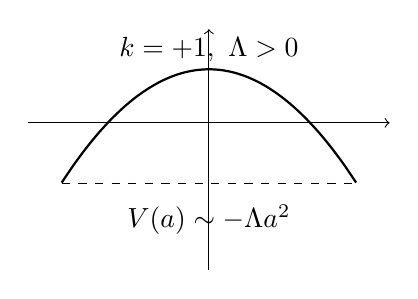
\begin{tikzpicture}[scale=0.85]
\draw[->] (-2.7,0) -- (2.7,0);
\draw[->] (0,-2.2) -- (0,1.4);
\draw[thick,domain=-2.2:2.2,smooth] plot (\x,{-0.35*(\x)^2 + 0.8});
\draw[dashed] (-2.2,-0.9) -- (2.2,-0.9);
\node at (0,-1.45) {\(V(a)\sim -\Lambda a^2\)};
\node at (0,1.1) {\(k=+1,\ \Lambda>0\)};
\end{tikzpicture}
\hspace{2em}
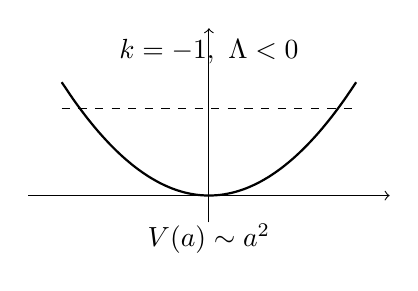
\begin{tikzpicture}[scale=0.85]
\draw[->] (-2.7,0) -- (2.7,0);
\draw[->] (0,-0.4) -- (0,2.5);
\draw[thick,domain=-2.2:2.2,smooth] plot (\x,{0.35*(\x)^2});
\draw[dashed] (-2.2,1.3) -- (2.2,1.3);
\node at (0,-0.65) {\(V(a)\sim a^2\)};
\node at (0,2.15) {\(k=-1,\ \Lambda<0\)};
\end{tikzpicture}
\caption{Potentiels effectifs schématiques pour le rebond de de Sitter fermé et l’effondrement d’un univers ouvert avec \(\Lambda\) négative.}
\label{fig:c05-mechanical-potentials}
\end{figure}

\begin{classroomqa}
\audiencequestion{Ces équations de Friedmann sont-elles vraiment les équations d’Einstein ?}
\lecturerresponse{Oui. Ce sont les équations de champ d’Einstein après que l’homogénéité et l’isotropie ont réduit la métrique à la seule fonction \(a(t)\). Cette réduction par symétrie élimine la plupart des composantes tensorielles et laisse cette équation différentielle ordinaire décrivant l’expansion cosmique. \lecturetimestamp{01:43:52--01:44:05}}
\end{classroomqa}

\begin{classroomqa}
\audiencequestion{Le facteur d’échelle \(a\) pourrait-il être complexe ?}
\lecturerresponse{Pas dans les cosmologies FRW classiques réelles étudiées ici. Le facteur d’échelle mesure la taille spatiale et est supposé réel et non négatif. Des géométries complexifiées peuvent apparaître dans d’autres approches mathématiques, mais elles n’interviennent pas dans les solutions de ce cours. \lecturetimestamp{01:44:06--01:44:21}}
\end{classroomqa}

\begin{classroomqa}
\audiencequestion{Y a-t-il une raison physique pour que la pression soit une fonction linéaire de la densité ?}
\lecturerresponse{Non. Une valeur constante de \(w\) est commode et décrit justement les principales composantes considérées ici. Un mélange de matière, de rayonnement et de vide n’a pas une valeur constante de \(w\) à toutes les époques, et un matériau général peut avoir une fonction \(P(\rho)\) non linéaire. Pour un fluide barotrope, \(dP/d\rho\) détermine le carré de la vitesse du son dans les unités où \(c=1\) ; une valeur constante de \(w\) rend cette dérivée constante, mais la nature n’est pas tenue de s’y conformer. \lecturetimestamp{01:44:21--01:45:34}}
\end{classroomqa}

\section{À retenir}

L’équation d’état relie la physique microscopique à l’évolution temporelle du facteur d’échelle. Le travail adiabatique dans une boîte comobile donne
\[
\rho\propto a^{-3(1+w)}.
\]
La matière froide a \(w=0\) et \(\rho\propto a^{-3}\). Le flux isotrope de quantité de mouvement des photons donne
\[
\left\langle\cos^2\theta\right\rangle=\frac13,
\qquad
P_{\mathrm r}=\frac{\rho_{\mathrm r}}{3},
\qquad
\rho_{\mathrm r}\propto a^{-4}.
\]

La tension rend physiquement intelligible une pression négative. Une densité de vide constante vérifie
\[
P_\Lambda=-\rho_\Lambda,
\qquad
w_\Lambda=-1.
\]
Une énergie du vide positive produit une expansion de de Sitter exponentielle dans le feuilletage plat et un rebond en \(\cosh\) dans le feuilletage fermé. Une énergie du vide négative peut entraîner la recontraction même d’un univers ouvert. Dans tous les cas de signe, l’équation de Friedmann peut se lire comme une équation d’énergie mécanique effective. La question qui reste sans réponse n’est pas pourquoi les champs quantiques contribuent à l’énergie du vide, mais pourquoi leur contribution nette observée est presque nulle sans l’être tout à fait.
